%%%%%%%%%%%%%%%%%%%%%%%%%%%%%%%%%%%%%%%%%%%%%%%%%%%%%%%%%%%%%%%%%%%%%%%%%%%%%%%%%%%%%%%%%%%%%%%%
%
% CSCI 1430 Written Question Template
%
% This is a LaTeX document. LaTeX is a markup language for producing documents.
% Your task is to answer the questions by filling out this document, then to
% compile this into a PDF document.
%
% TO COMPILE:
% > pdflatex thisfile.tex
%
% If you do not have LaTeX and need a LaTeX distribution:
% - Departmental machines have one installed.
% - Personal laptops (all common OS): http://www.latex-project.org/get/
%
% If you need help with LaTeX, come to office hours. Or, there is plenty of help online:
% https://en.wikibooks.org/wiki/LaTeX
%
% Good luck!
% James and the 1430 staff
%
%%%%%%%%%%%%%%%%%%%%%%%%%%%%%%%%%%%%%%%%%%%%%%%%%%%%%%%%%%%%%%%%%%%%%%%%%%%%%%%%%%%%%%%%%%%%%%%%
%
% How to include two graphics on the same line:
%
% \includegraphics[width=0.49\linewidth]{yourgraphic1.png}
% \includegraphics[width=0.49\linewidth]{yourgraphic2.png}
%
% How to include equations:
%
% \begin{equation}
% y = mx+c
% \end{equation}
%
%%%%%%%%%%%%%%%%%%%%%%%%%%%%%%%%%%%%%%%%%%%%%%%%%%%%%%%%%%%%%%%%%%%%%%%%%%%%%%%%%%%%%%%%%%%%%%%%

\documentclass[11pt]{article}

\usepackage[english]{babel}
\usepackage[utf8]{inputenc}
\usepackage[colorlinks = true,
            linkcolor = blue,
            urlcolor  = blue]{hyperref}
\usepackage[a4paper,margin=1.5in]{geometry}
\usepackage{booktabs}
\usepackage{stackengine,graphicx}
\usepackage{fancyhdr}
\setlength{\headheight}{15pt}
\usepackage{microtype}
\usepackage{times}
\usepackage{amsmath}

% python code format: https://github.com/olivierverdier/python-latex-highlighting
%\usepackage{pythonhighlight}

\frenchspacing
\setlength{\parindent}{0cm} % Default is 15pt.
\setlength{\parskip}{0.3cm plus1mm minus1mm}

\pagestyle{fancy}
\fancyhf{}
\lhead{Final Project}
\rhead{DATA 1030}
\rfoot{\thepage}

\date{}

\title{\vspace{-1cm}Automatic Human Sleep Stage Classification through Machine Learning}
\author{Zhiyan Wang}


\begin{document}
\maketitle
\vspace{-1cm}
\thispagestyle{fancy}

\section*{Introduction}
Sleep is ubiquituous in human and plays a critical role in human development, emotional regulation, learning and memory. Sleep can largely be charaterized into NREM sleep and REM sleep. REM sleep is the stage in which dreaming occurs. NREM sleep can be further characterized into N1, N2 and N3 based on the depth of he sleep.N3 sleep is also known as slow wave sleep which is the deepest sleep stage of each participant.  Different sleep stages and sleep components in different frequencies have been associated with different functions of sleep. Under experimental circumstances, sleep is measured using polysomnfography(PSG) which contains EEG for brain waves, EMG for muscle tone and EOG for eye movement. For every sleep research, one of the first steps is to characterize the subject's sleep into different sleep stages with visual examination. Different sleep stages are characterized by different frequencies of EEG waves and different patterns of eye movement. A human experimentor will incorportate the patterns and label each sleep epoch with a stage label according to the manual\cite{sleepmanual}. The process is largely based on experience, which makes sleep staging inaccurate and subjective. 

The motivation of the current project is to use machine learning techniques to help achieve the goal of automatically characterizing sleep stages.  

\section*{Datasets}
\begin{itemize}
\item The data were collected using polysomnography with a length of 90 minutes for the nap. 90 minutes is usually the length of a full sleep cycle in afternoon nap. The sleep typically develops from N1, to N2 and to N3. Then subjects will go from N3 to N2 and N1 and has a sudden transfrom to REM sleep. I have six participants with 2 naps each. For traditional sleep scoring, we would select score 30s window from the data and label the 30s data with a sleep stage. The labels were previously created with bare eye of an experienced experimenter. 
\item I used fast fourier transformation(fft) from MNE-python package \cite{mne} to preprocess the data. I took the 30s epoch and applied fft to the data. Then I obtained a power for the following frequency band for each epoch: alpha (10-12hz), theta(4-7hz), delta(1-4hz), sigma(12-20hz). Different sleep stage could be associated with different featuring frequency bands. For example, N1 and REM are characterized by theta activity. N3 is characterized by delta activity and so on. The data were stored in a dataframe with columns, alpha, theta, delta, sigma, label(sleep stage), EEG channel, subject, nap(with or without sleep). The episodes with artifacts have been marked with nan values. Label was encoded with label encoder. 
\end{itemize}

\section*{Exploratory Data Analysis}
\begin{itemize}
\item \textbf{Correlation among features} \\
The correlation coefficient between feature label paris have been plotted as Figure ~\ref{fig:corrs} below. The 10 strongest positive correlations were observed among different frequencies of brain waves and the sleep stage label(alpha, theta, slow wave and sigma). \\
\begin{figure}[h!]
  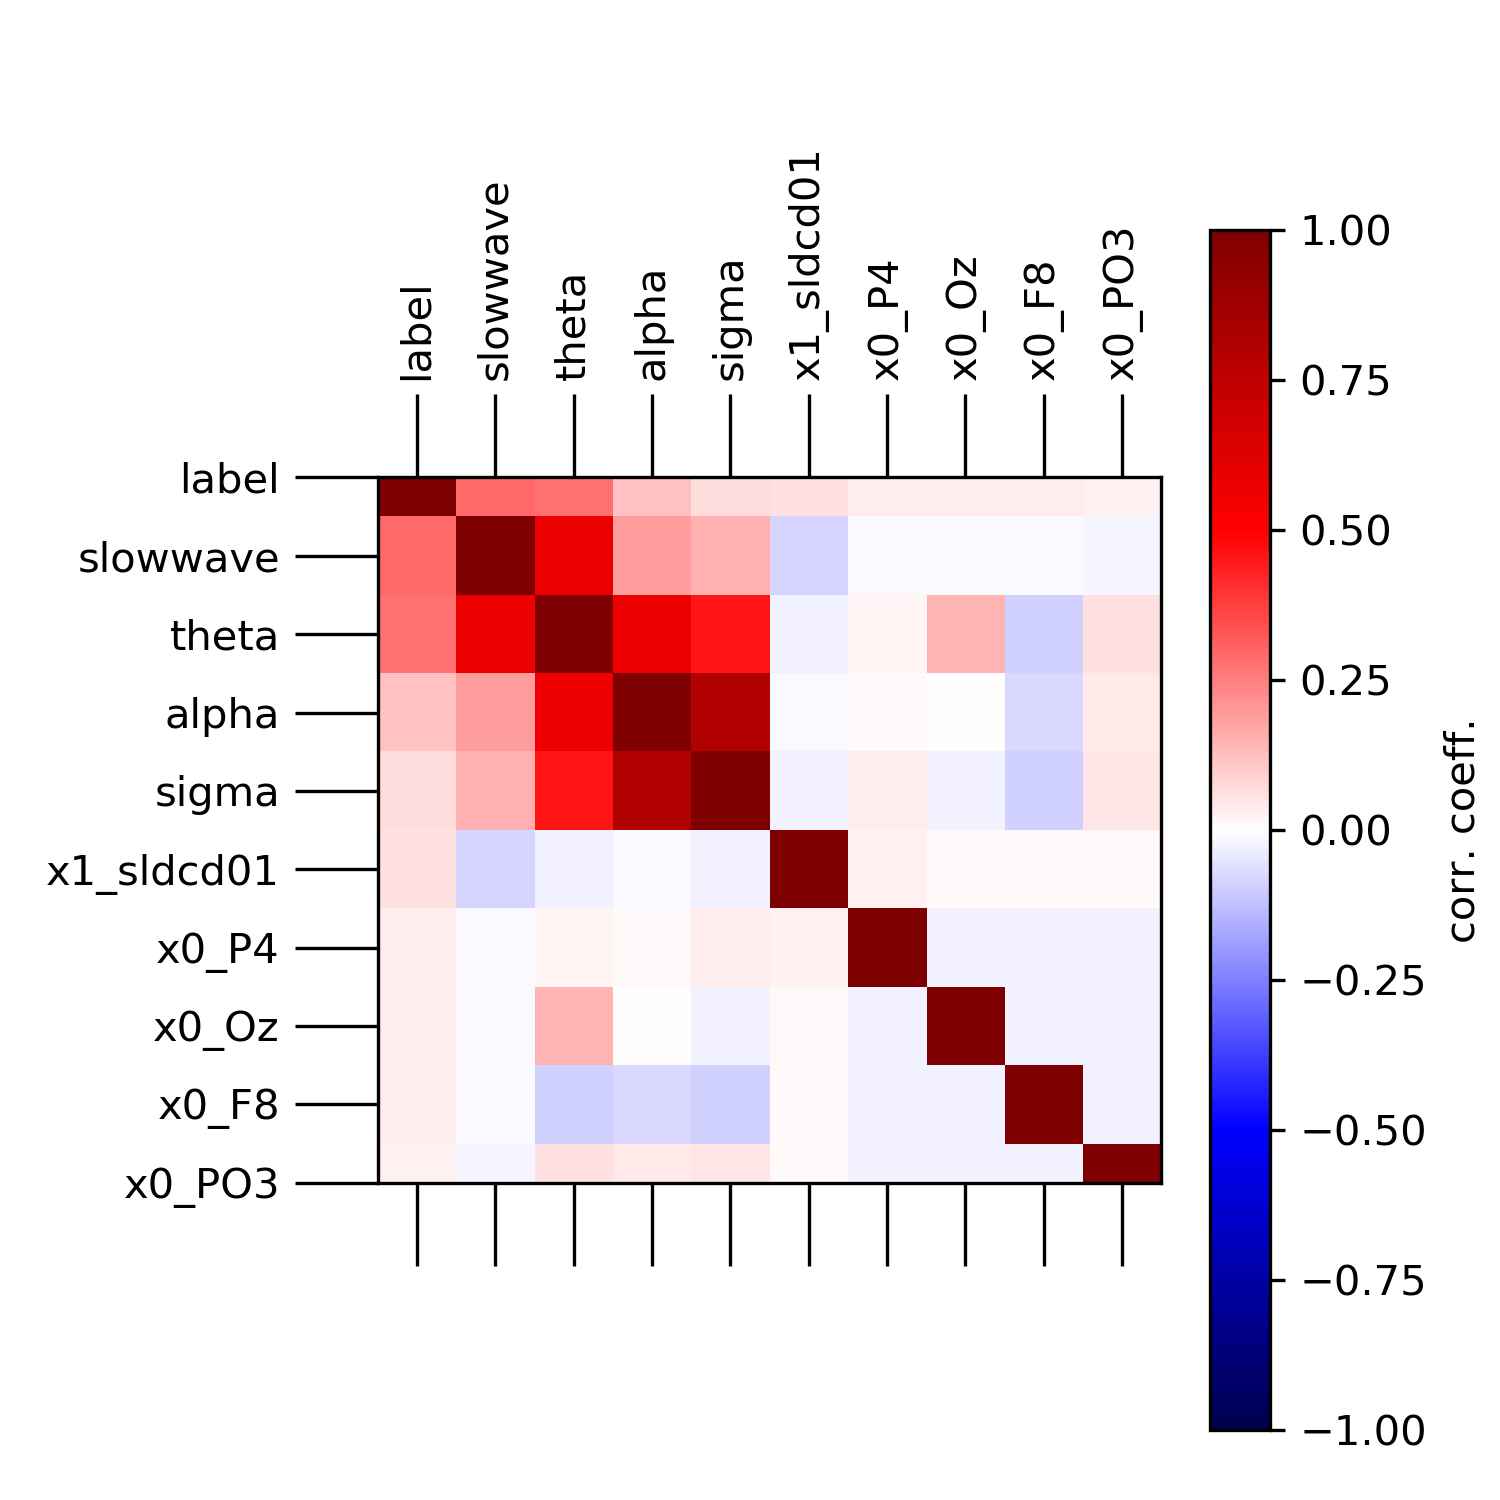
\includegraphics[width=0.9\textwidth]{corr_coeff_dummies_poscorr}
  \caption{Top 10 Cross-Correlation coefficient between features}
  \label{fig:corrs}
\end{figure}

\item \textbf{Scatter Matrix of highly correlated features and label}
To observe the data more carefully, we obtained the scatter matrix of different frequencies and how they covariate with other frequencies grouped by different sleep stage lable. Figure ~\ref{fig:scatter} demonstrated that frequencies show different patterns for different sleep stage when compared with other frequencies.\\
\begin{figure}[h!]
  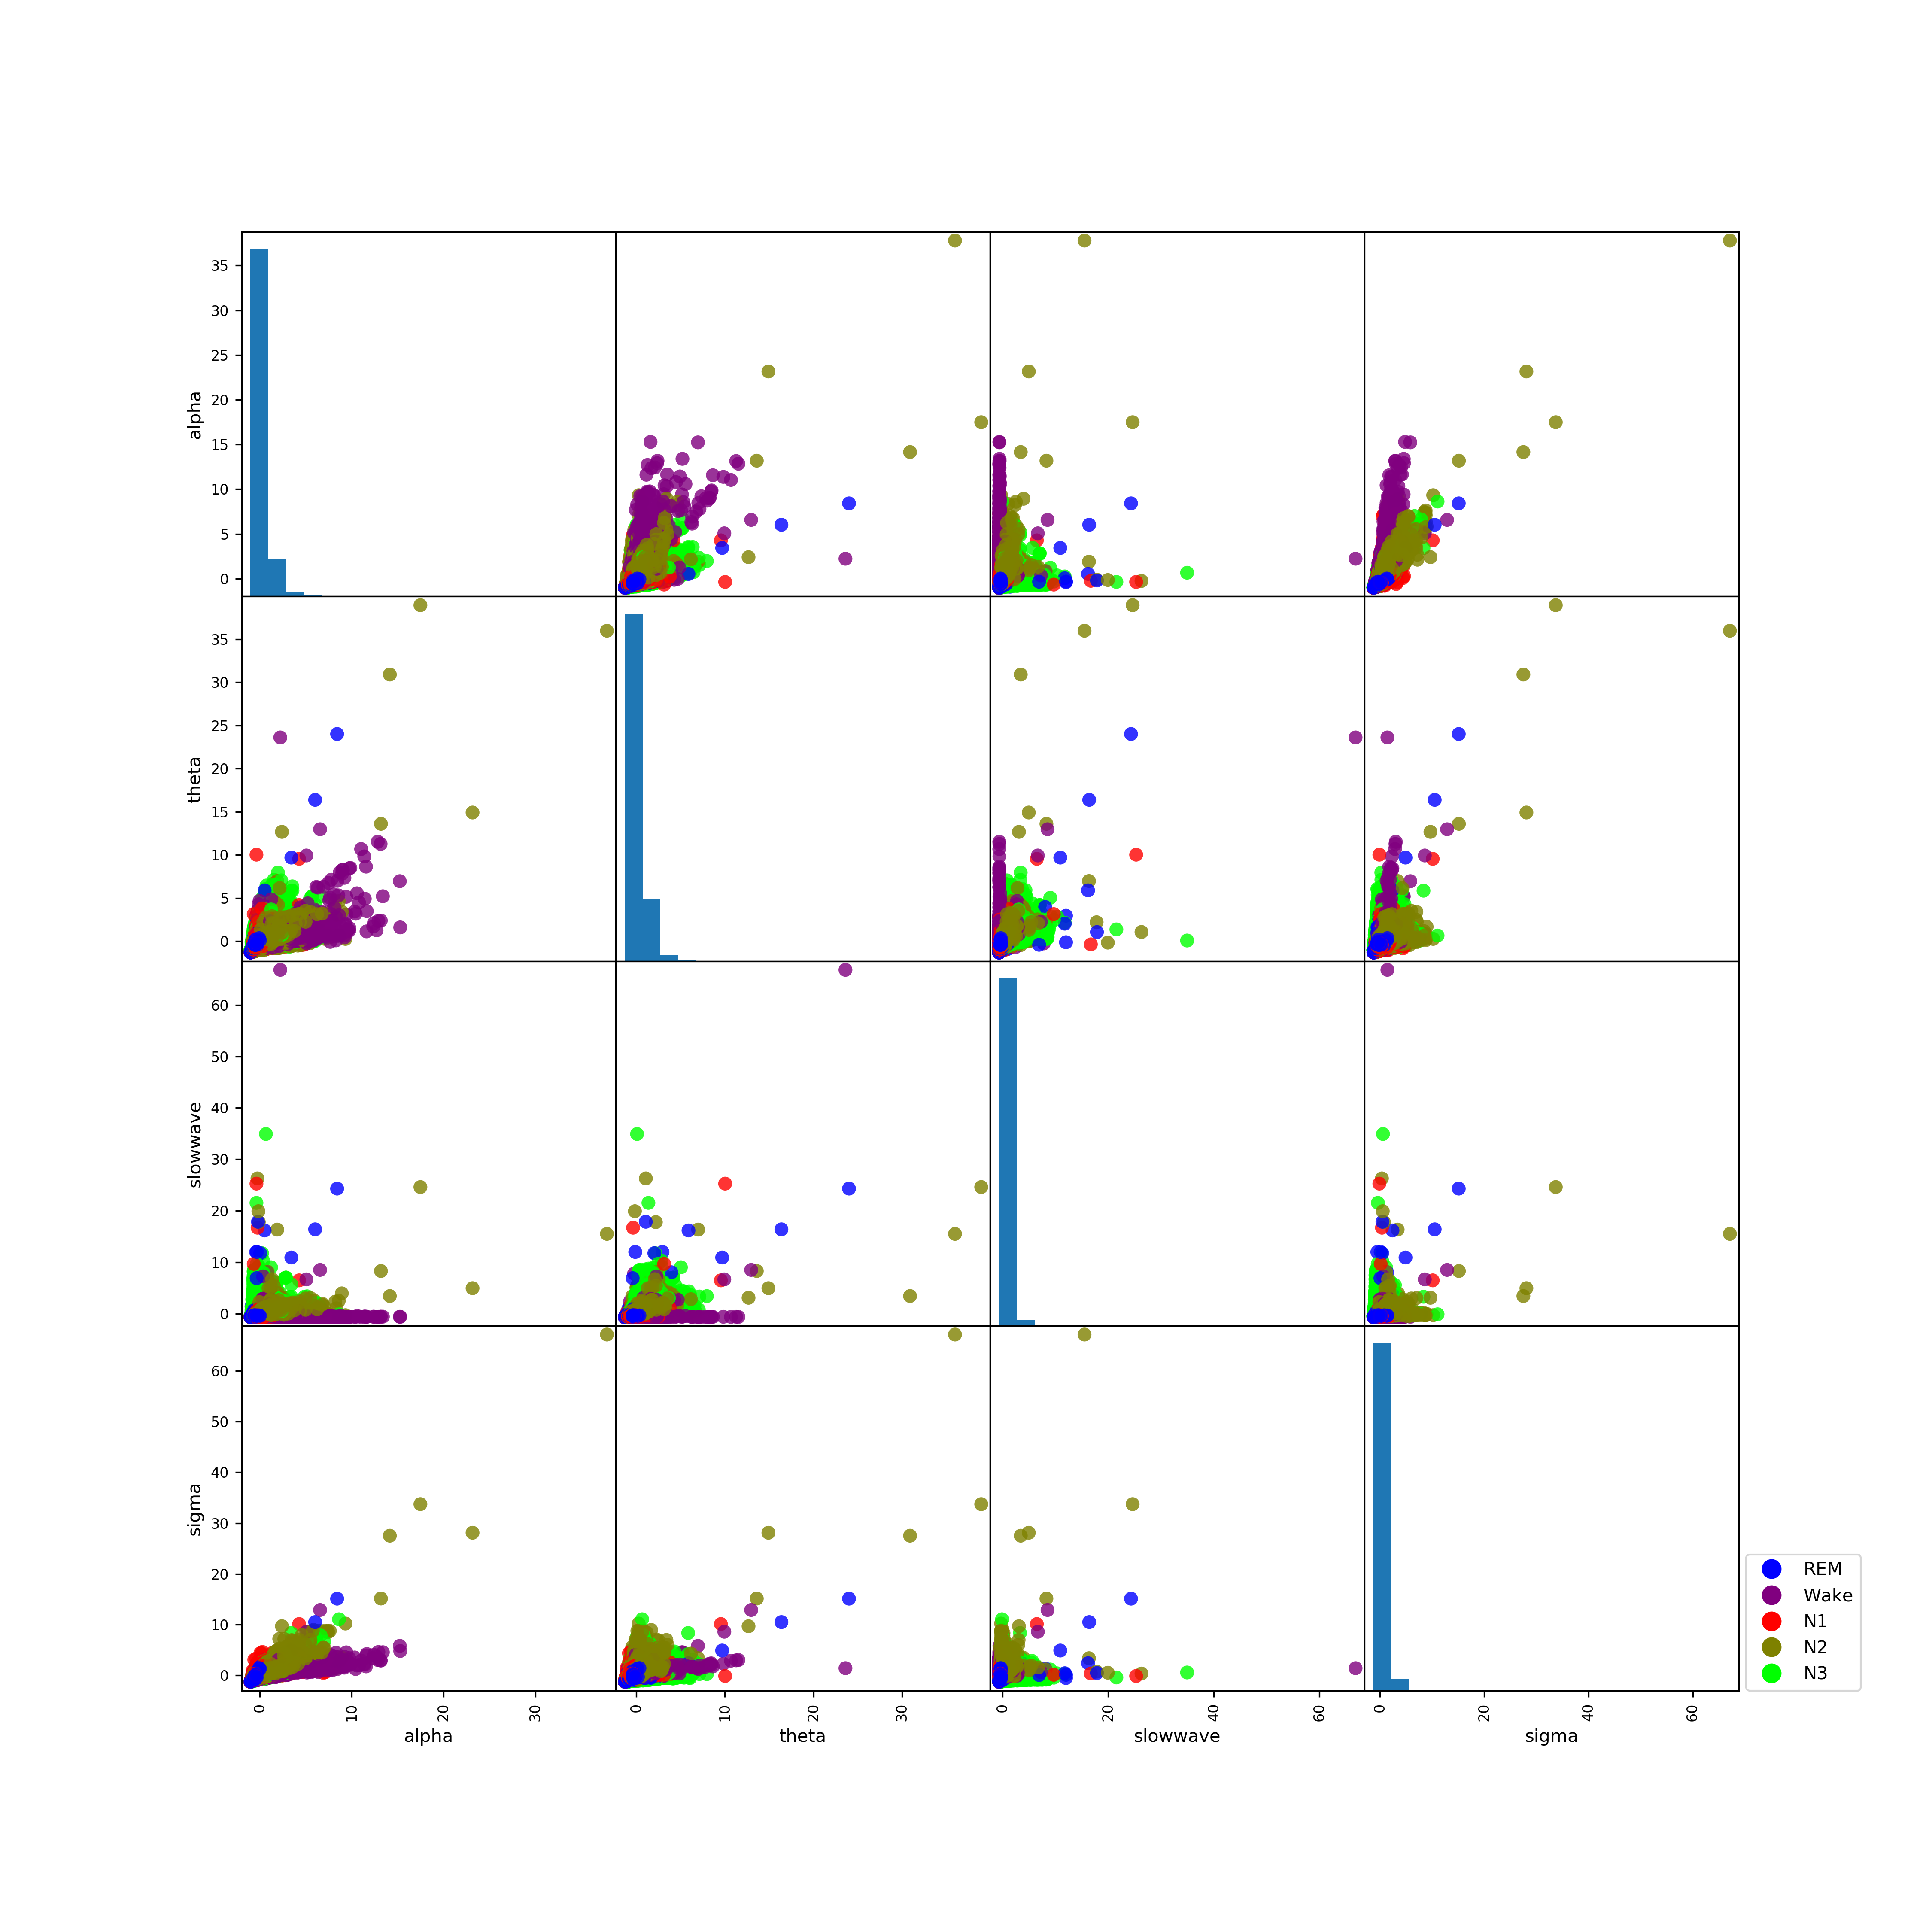
\includegraphics[width=0.9\textwidth]{scattermatrix}
  \caption{Scatter Matrix of Different Frequencies Group by Sleep Stage Label}
  \label{fig:scatter}
\end{figure}
\item \textbf{Boxplot for individual feature}
We further obtained the boxplot in Figure ~\ref{fig:boxplot} for each individual feature grouped by different sleep stage. The outlier were the imputed missing values which will be discussed later. \\
 \begin{figure}[ht]
  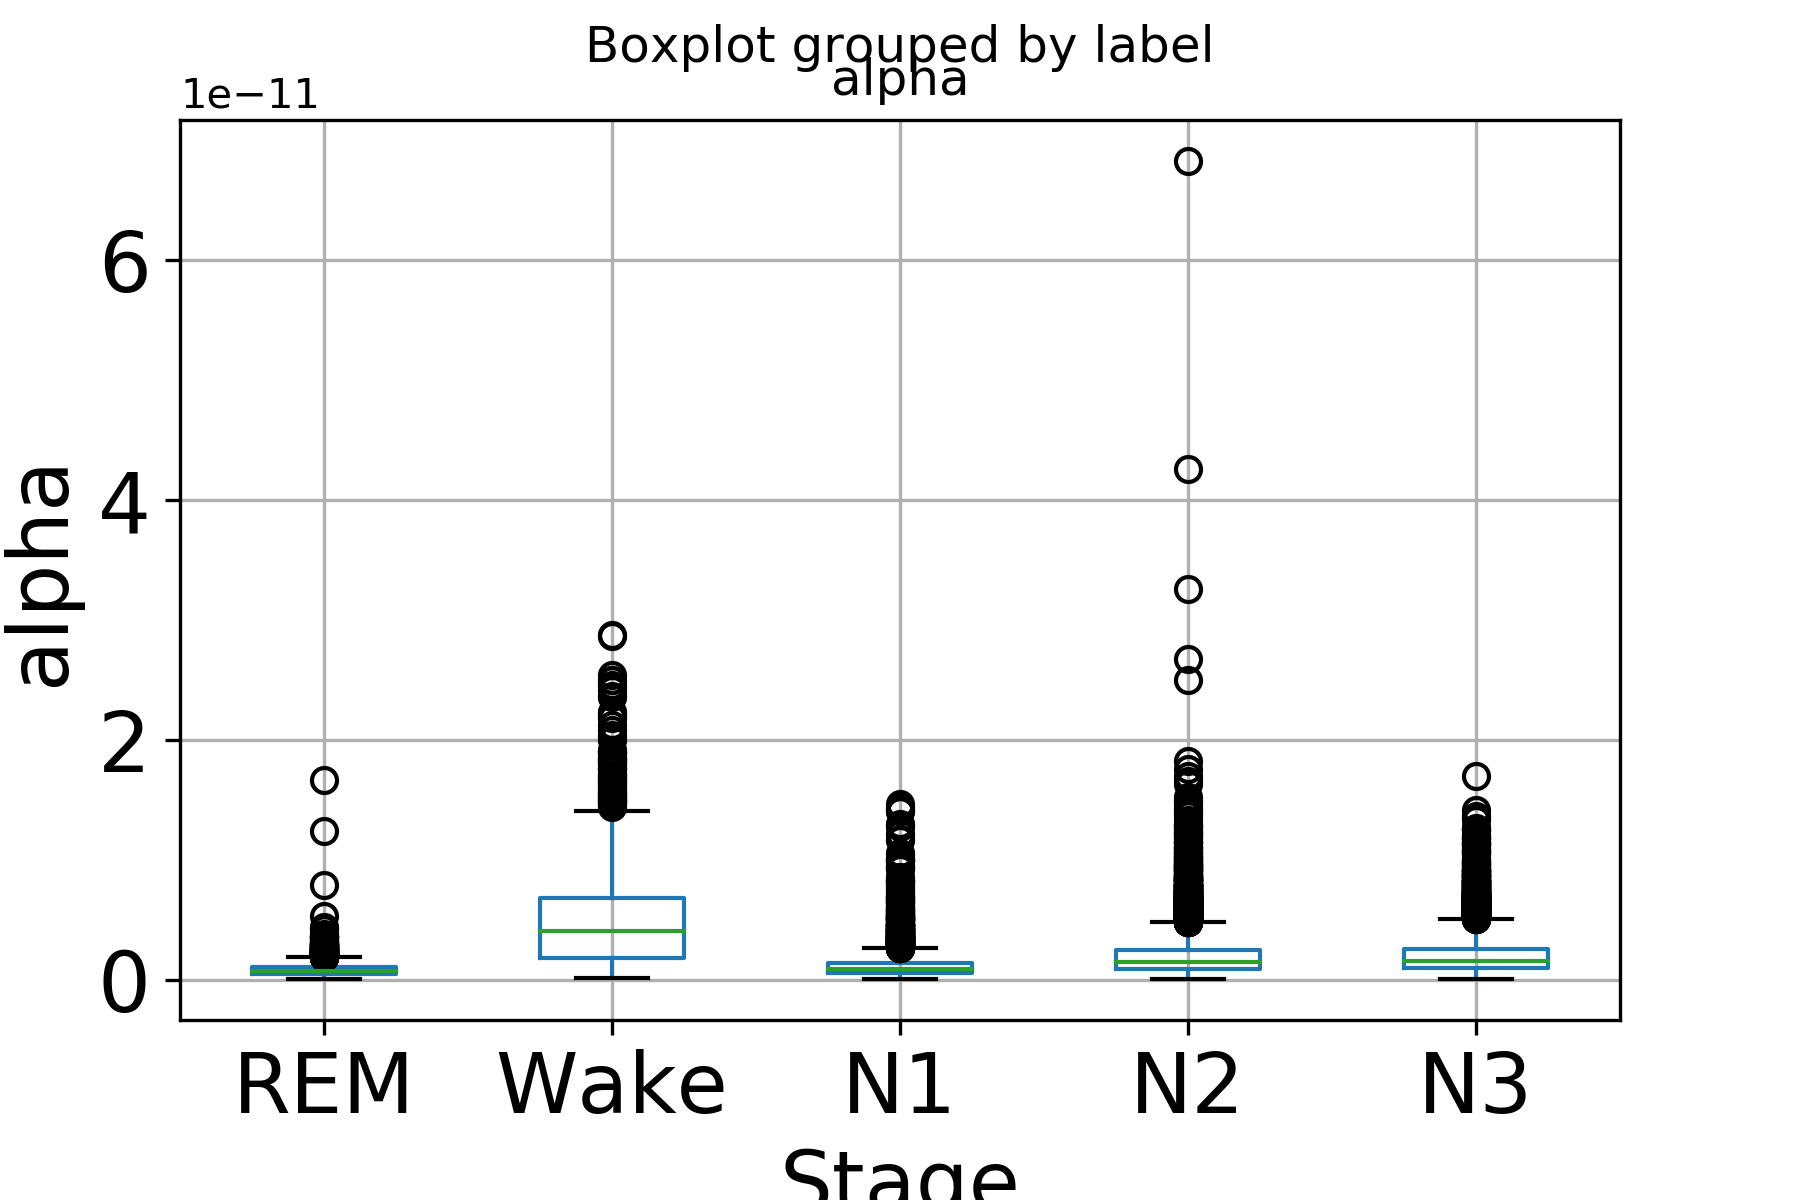
\includegraphics[width=0.45\textwidth]{boxplotalpha}
  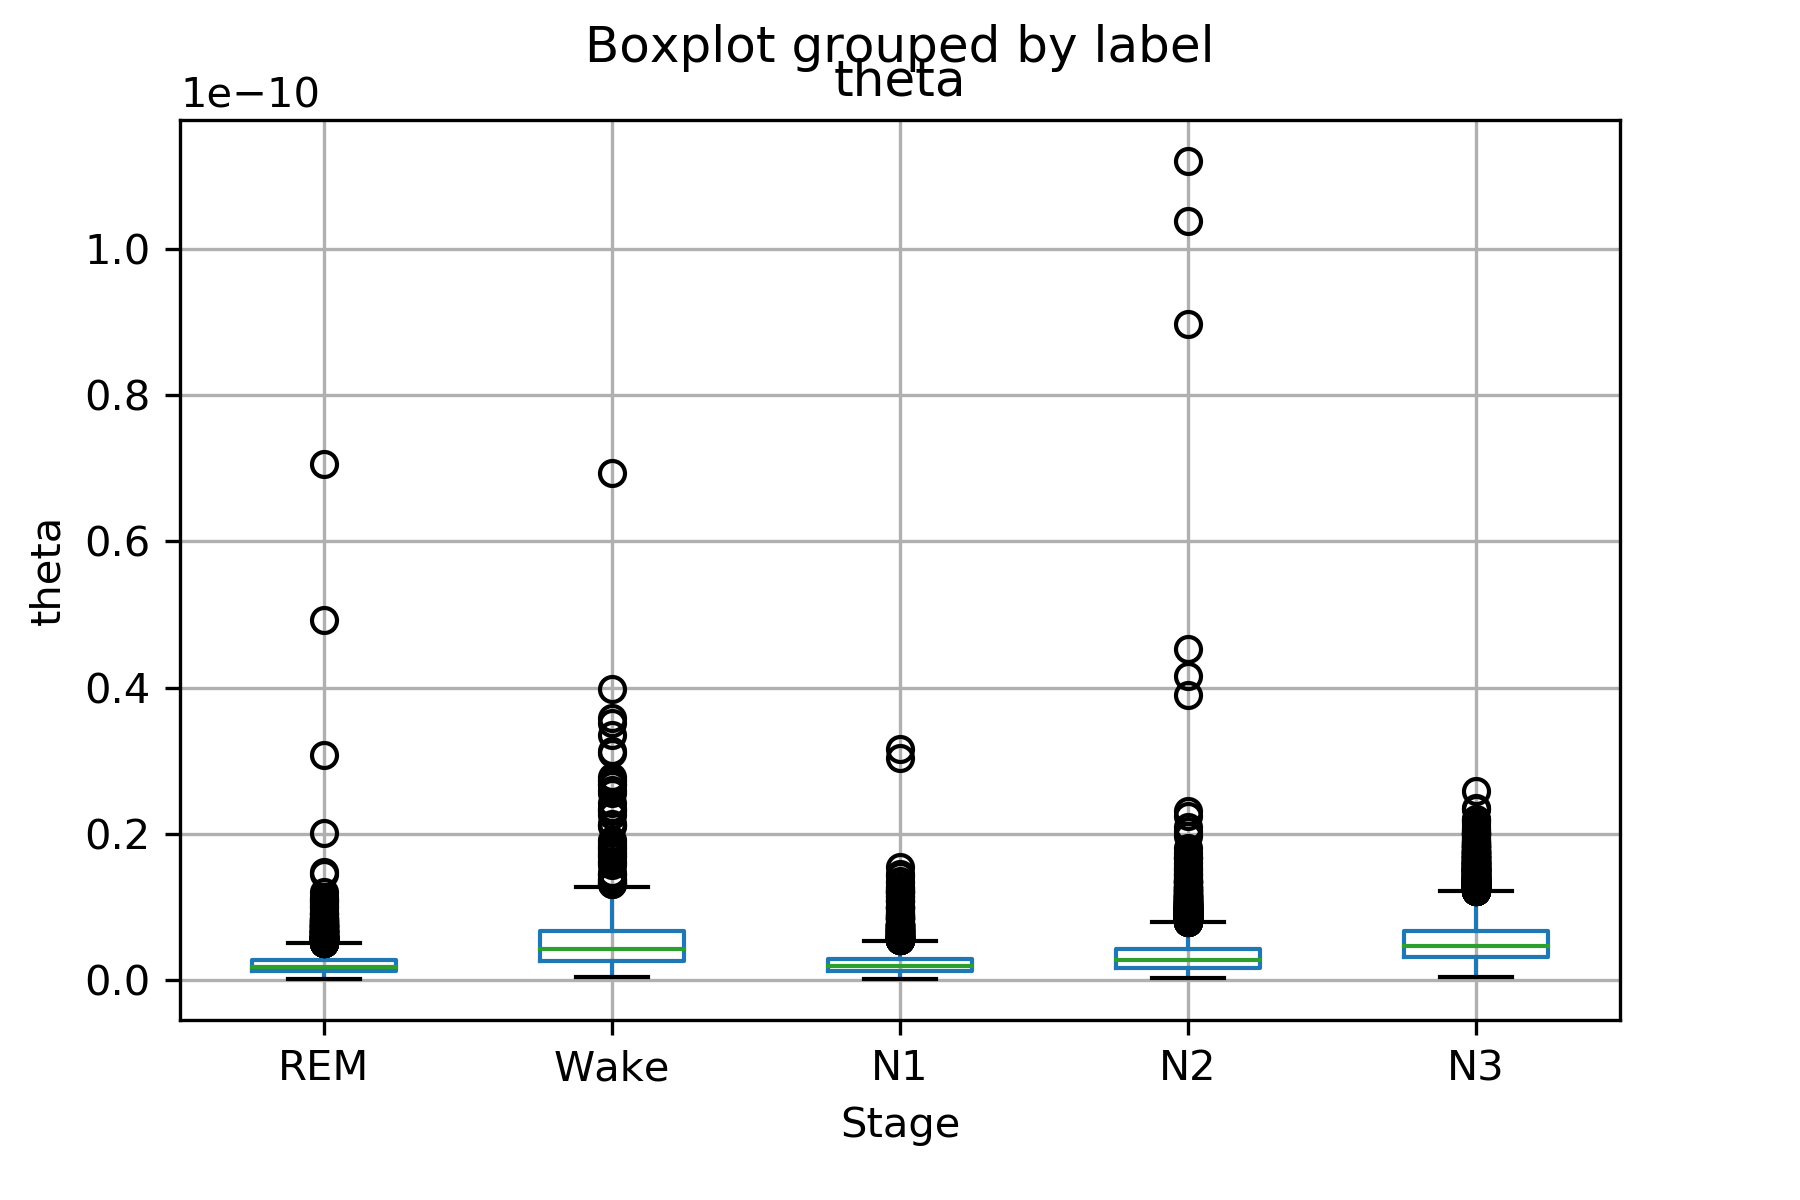
\includegraphics[width=0.45\textwidth]{boxplottheta}
  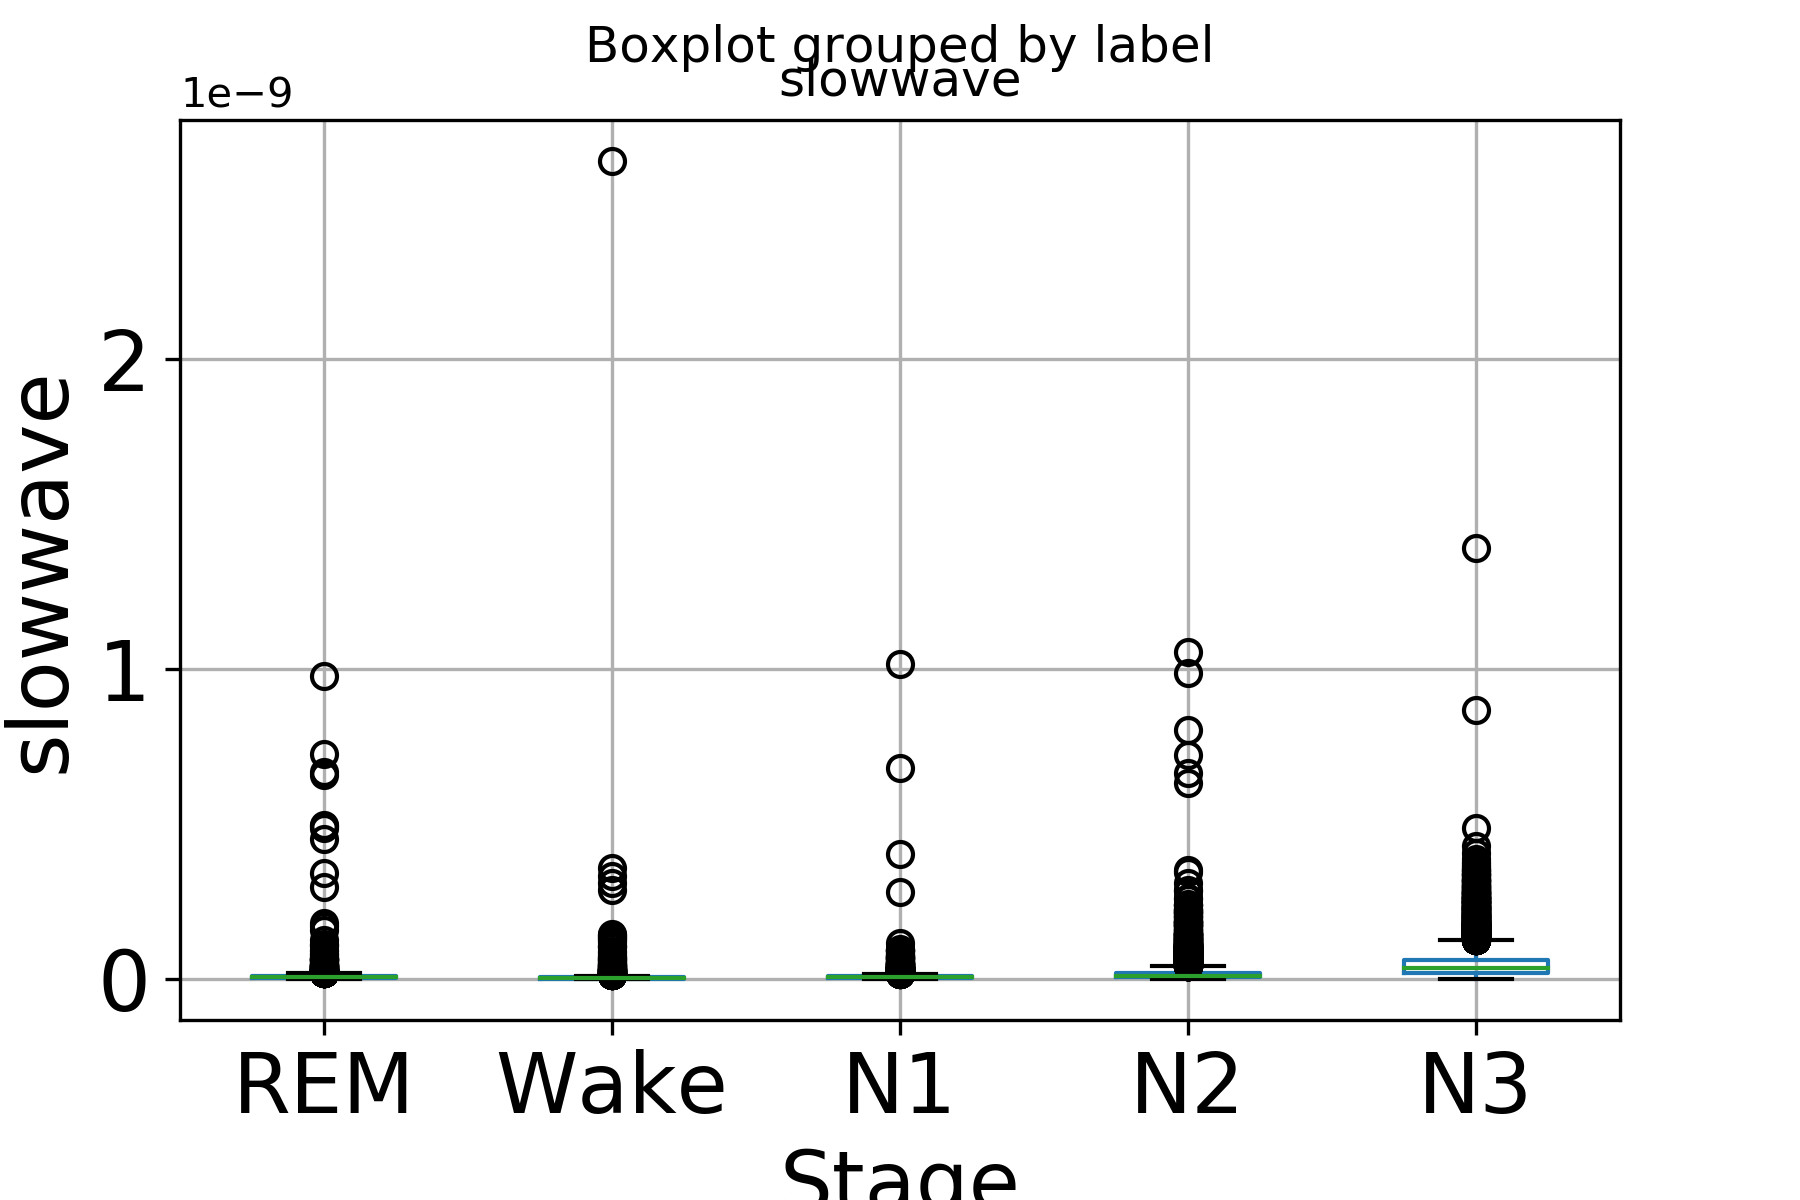
\includegraphics[width=0.45\textwidth]{boxplotslowwave}
  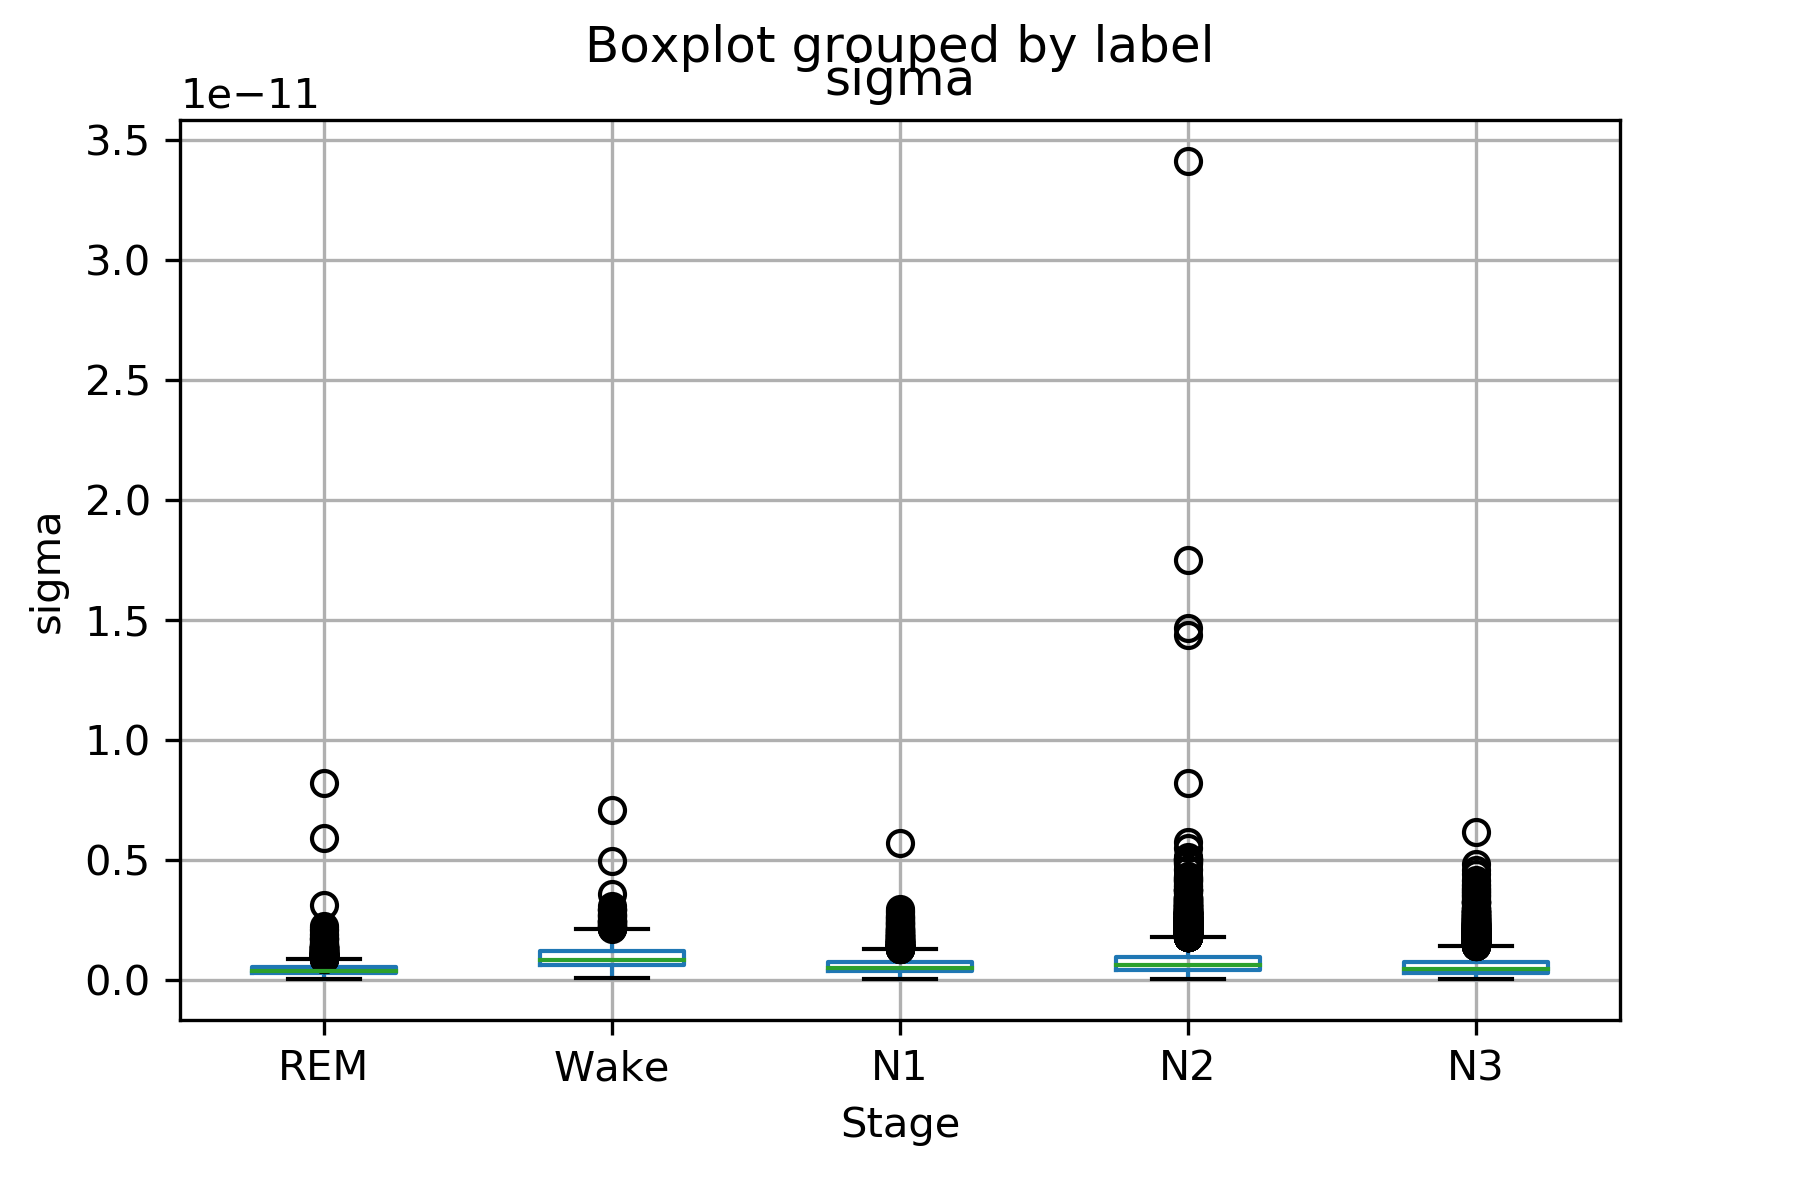
\includegraphics[width=0.45\textwidth]{boxplotsigma}
  \caption{Boxplot of Different frequencies}
  \label{fig:boxplot}
\end{figure} 
\end{itemize} 

\section*{Methods}
Subject ID and Nap would be used to group the data points and was thus dropped from the features. The features used were, alpha, theta, sigma, slowwave and electrodes(categorical).\\ 
\\
A total of three algorithms have been applied to the dataset: Random Forest, Logistic Regression and XGBoost. Logistic Regression was applied based on the fact that this is a classfication problem and logistic regresson is the simplest model for such probelm. Different features in this problem can be separated into different steps or categories in determining sleep stages if a human were to classify the sleep stage. For instance, high alpha and high theta would be N1 and high slowwave would be N3. Thus, random forest is applied. XGBoost was applied to obtain a more reasonable estimation of missing values. Models were evalued based on accuracy. The variability of the model estimation was measured by repeating each model 5 times with different random state and obtain the mean accuracy and standard deviation of model estimation. \\
\\
The pipeline of Random Forest and Logistic Regression is shown in Figure ~\ref{fig:mlpipeline1}. Data was first split into test, Cross validation(CV) and training sets. Here Group-2-fold was used some data are from the same participant either in nap2 and nap3. The group is an dex of permutation of subject IDs and nap IDs. 2-fold was used to save computation time. Here simple imputer was used for both categorical and standard scalar features. Iterative imputer generated outliers for the data as shown in Figure ~\ref{fig:boxplot}. As the variance across brain wave amplitude is very small across people and across different electrodes, we used simple imputer, namely the mean to substitue the missing data. This is not ideal, but it will give us an idea of how well the model performs. The best hyperparameter was selected as the output of the model. 5-fold cross validation was also performed but no difference was observed. The hyperparameters range is shown in Table ~\ref{tab:hyper}\\
\begin{figure}[ht]
  \includegraphics[width=0.9\textwidth]{imputepipe}
  \caption{Machine Learning pipeline for Random Forest and Logistic Regression}
  \label{fig:mlpipeline1}
\end{figure} 
\\
The pipeline of XGBoost is shown in Figure ~\ref{fig:xgboost}. The difference is that no missing value imputation was performed. reg\_alpha was hyper tuned for model performance as shown in Table ~\ref{tab:hyper}. 
\begin{figure}[ht]
  \includegraphics[width=0.9\textwidth]{xgboost}
  \caption{Machine Learning pipeline for XGBoost}
  \label{fig:xgboost}
\end{figure} 


\begin{table}[hb]
\centering
\caption{Hyperparameters} 
\begin{tabular}{ c c c }
 \textbf{Model} & \textbf{Hyperparameter} & \textbf{values} \\ 
 Random Forest & max\_depth, num\_estimators & 5 logscaled number[1, 1000],5 integers between [1,5] \\  
 Logistic Regression & alpha & 5 logscaled number[0.01, 100]\\
 XGBoost & alpha & 5 logscaled number[0.01, 100]
\end{tabular}
\label{tab:hyper} 
\end{table}

\section*{Results}
The baseline accuracy of the model is 0.34 for the portion of N2 sleep. We compared the performance of the three models in Table ~\ref{tab:result} below. The highest accuracy was obtained by random forest. However, XGBoost is more reasonable with regard to missing value. Moreover, all of the models have accuracy way above the baseline and there is no significant difference between these models. The best model in this regard would be XGBoost. \\
\\
Therefore, our model would be XGBoost model. We calcualted feature importance by performing permutation tests on each of the features using the best model we obtained with hyperparameter alpha equals to 1. The result is shown in Figure ~\ref{fig:permutation}. \\
\\
The most important features are slow wave and sigma. This makes sense in the academic setting as slow wave is characteristic of N3 sleep and sigma is characterized of N2 sleep. Moreover, these two stages constittute of around 60\% of the datapoint. alpha and theta are less important as alpha and theta are equal likely in N1 and REM sleep. Channel number are least important as for different stages and components, it's rather homogeneous across different channels of the EEG recording device.\\  

\begin{figure}[ht]
  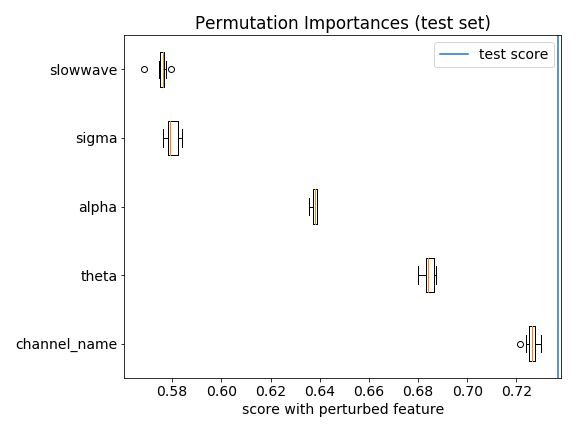
\includegraphics[width=0.9\textwidth]{feature_permutation}
  \caption{Feature Importance by Permuation}
  \label{fig:permutation}
\end{figure} 

\begin{table}[ht]
\centering
\caption{Results of Different Models} 
\begin{tabular}{ c c c }
 \textbf{Model} & \textbf{Mean Accuracy} & \textbf{Standard Deviation (+/-)} \\ 
 Random Forest & 0.63 & 0.06 \\  
 Logistic Regression & 0.67 & 0.04\\
 XGBoost & 0.64 & 0.06
\end{tabular}
\label{tab:result} 
\end{table}

\section*{Outlook}
Although the current exceeds the baseline accuracy of the model, it's still not appropriate for applications in academic setting. According to the feature importance result, the model might be useful for determining NREM(N2+ N3) versus other stages rather than characterizing all of the sleep stages. One feature that distinguish REM and N1 sleep is the amplitude of muscle tone which is close to zero during REM. The current data does not include the muscle tone data. For better results, muscle tone data might provide extra information to distinguish between REM and other sleep stages. Furthermore, there is another possibility that the problem might be innately hard for the machine learning algorithms we discussed here. To obtain a better accuracy, a more complexed model like Neural Networks might be necessary. In that case, we can not only use the transformed tabular format data, but also the original epochs in time domain. More information and more complexed models might improve the accuracy of classifying of human sleeps automatically. This would potentially be beneficial not only to the academic setting but also to empirical usage such as sleep tracking devices. (1195/2000 words)
\\

\textbf {Github} \\ 
The repository \href{https://github.com/zhiyanwang27/decoding_sleep}{link} \textbf{PLEASE DO NOT DOWNLOAD THE DATA OR SHARE WITH ANYONE ELSE, THANK YOU !!!} 
\begin{thebibliography}{9}
\bibitem{sleepmanual}
Berry, R. B., Brooks, R., Gamaldo, C. E., Harding, S. M., Marcus, C., Vaughn, B. V. (2012). \textit{The AASM manual for the scoring of sleep and associated events.} Rules, Terminology and Technical Specifications, Darien, Illinois, American Academy of Sleep Medicine, 176.

\bibitem{mne}
A. Gramfort, M. Luessi, E. Larson, D. Engemann, D. Strohmeier, C. Brodbeck, L. Parkkonen, M. Hämäläinen. (2014). \textit{MNE software for processing MEG and EEG data, NeuroImage, Volume 86, Pages 446-460, ISSN 1053-8119}. 
 
\end{thebibliography}


 
\end{document}



